\documentclass[10pt,a4paper]{article}
\usepackage[utf8]{inputenc}
\usepackage[english]{babel}
\usepackage{amsmath}
\usepackage{amsfonts}
\usepackage{amssymb}
\usepackage{graphicx}
\author{Markus Meier}
\title{Heuristic Analysis}

\begin{document}
\maketitle

\section{Heuristic 1}
The idea behind this heuristic is that it is advantageous for the player to choose board states that allow him more moves in his next turn.

\section{Heuristic 2}
The idea behind this heuristic is that it is advantageous for the player to limit the freedom of his opponent. That means the less moves the opponent has the better for the player. This might be scaled with a certain aggressive factor.

\section{Heuristic 3}
This heuristic tries to combine the first two approaches.

We count for both players the available moves.
However, moves that lead close to the border of the game board are penalized,
since they will have less freedom in the following steps of the game.

\section{Evaluation}
On the following pages, there are some screenshots from the evaluations in three tournaments. The results are not consistent for all the scores, so it is hard to tell if heuristic 3 is really better. More samples could solve the issue, but require more time.


\begin{figure}
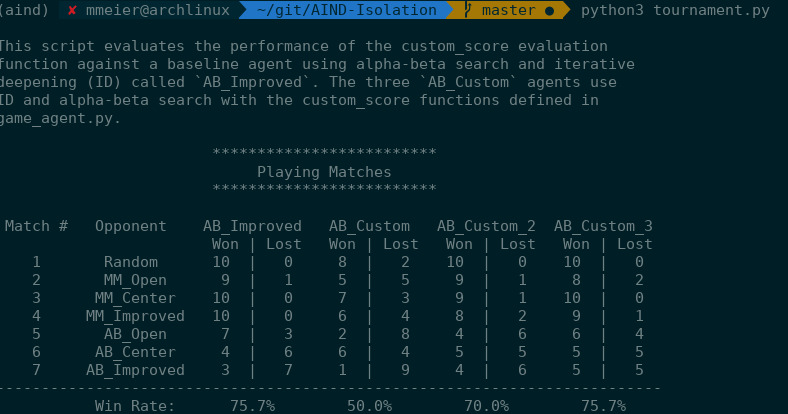
\includegraphics[scale=0.5]{image1.jpg}
\end{figure}

\begin{figure}
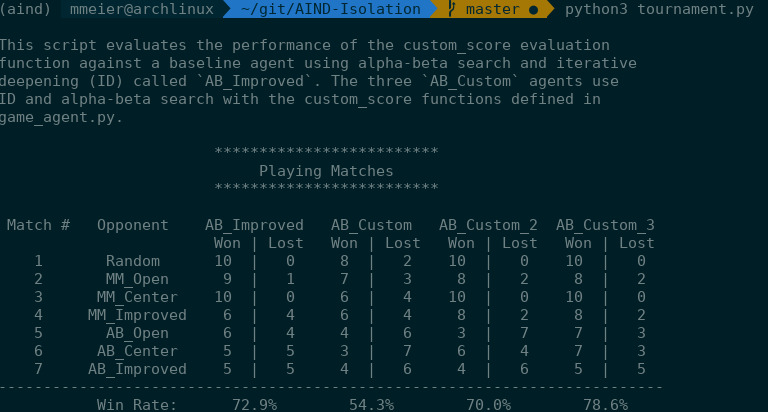
\includegraphics[scale=0.5]{image2.jpg}
\end{figure}

\begin{figure}
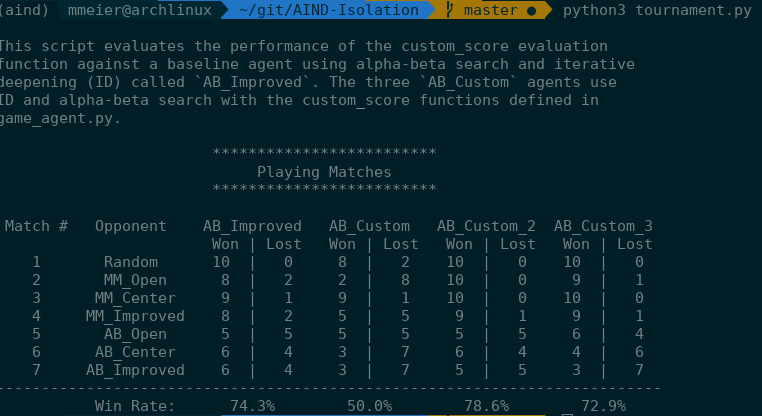
\includegraphics[scale=0.5]{image3.jpg}
\end{figure}

\end{document}